\documentclass[xcolor=dvipsnames]{beamer}
%\usecolortheme[named=RoyalBlue]{structure}
%\usecolortheme[named=CornflowerBlue]{structure}
\usecolortheme[named=Red]{structure}
%\usetheme{Antibes}
\usetheme{Singapore}
%\usetheme{Berlin}
\usepackage[spanish, activeacute]{babel}
\usepackage[latin1]{inputenc}
\usepackage{times}
\usepackage[T1]{fontenc}

\usepackage{graphicx}

\setbeamertemplate{blocks}[shadow=true] 
\setbeamertemplate{navigation symbols}{} 

\title[Control de Versiones]{Nuevo enfoque de versionamiento para desarrollo}
\author{Esteban Gomez, Jorge Medina - Santiago/Chile}

\institute{ADEM Ltda. - Grupo Empresas JP \scriptsize{\textcircled{\tiny{R}}}}
%\mode<presentation>

\date{Agosto. 28 , 2009}

\AtBeginSection[]
{
	\begin{frame}<beamer>
		\frametitle{Index}
		\tableofcontents[currentsection]
	\end{frame}
}

\begin{document}
\fontsize{7}{9}
	\begin{frame}
		\titlepage
	\end{frame}
	
\section{Introducci\'on}
	\begin{frame}{Introducci'on}
	\scriptsize
	{
	\begin{tabbing}	
	Que es subversi'on? \\ \\
	Es un sistema de control de versiones de c'odigo abierto bajo licencia Apache,		\\
	capaz de manejar archivos y directorios, controlando los cambios que estos sufren 	\\
	en el tiempo. \\ \\
	Para qu'e sirve subversi'on?\\ \\
	Dada la explicaci'on lo anterior permite examinar la historia de los archivos versionados\\
	bajo este sistema de control.\\ \\
	
	Por lo tanto se puede tener en el:\\ 
	La documentaci'on, el c'odigo fuente, ejecutables. etc. \\
	Todo lo anterior y mucho m'as, con un completo historial de modificaciones.\\
	\end{tabbing}
	}
	\end{frame}
	
	\begin{frame}{Beneficios}
	\scriptsize
	{
	\begin{itemize}	
	\item Trabajo concurrente de m'ultiples programadores en un mismo proyecto directorio o archivo.
	\item Detecta los conflictos y evita que se sobre escriban los archivos reduciendo los accidentes
	 de sobre escritura de estos.
	\item Permite tener estadist'{i}ca de las modificaciones y las lineas modificadas.
	\item Integrar un sistema de ticket y de seguimiento de errores en el desarrollo de los proyectos.
	\item Es la forma m'as optima de llevar el desarrollo de sistemas.
	\item Maneja eficientemente las versiones en archivos de texto como binarios.
	\item Almacena los cambios de manera incremental en binarios y textos.
	\item Permite recuperar versiones o archivos anteriores sin necesidad de 
		recurrir al operador o administrador de los sistemas.
	\item Ayudara en la eliminacion del uso de super usuario.
	\item Accesos de solo lectura o lectura/escritura por ruta de acceso.
	\item Cliente multiplataforma.
	\end{itemize}
	}
	\end{frame}
	
	\begin{frame}{Problem'atica}
	\scriptsize
	{
	\begin{itemize}
	\item Representa un cambio de costumbre.
	\item Requiere capacitaci'on de los desarrolladores (tiempo)
	\item Requiere modificar la estructura actual.
	\item Requiere revisi'on exhaustiva de los sistemas.
	\item Resistencia a eliminar el versionamiento actual de ADEM SISTEMAS \\
		(rm -rf *.cb?[0-9]*)
	\end{itemize}
	}
	\end{frame}

	\begin{frame}{Por qu'e?}
	{
	\begin{itemize}
	\item Es el primer y m'as importante paso en la reingenier'{i}a de 
			operaciones (Desarrollo/Respaldos/QA/BI/etc.)
	\item Para hacer del servidor de desarrollo un repositorio oficial \\
			de todos los proyectos de la empresa.
	\item Entragar informaci'on cuantificable sobre los proyectos.
	\item Permite monitoriar el trabajo de los desarrolladores.
	\item Puede medir cuanto c'odigo escribe a diario un programador.
	\item Se puede obtener la diferencia exacta del codigo que se midifico.
	\item Una vez respaldado el repositorio de c'odigo, los esfuerzos de 
		  respaldos se centran en los archivos transaccionales no en el c'odigo fuente.
	\item Genera menos trabajo y esfuerzo en respaldos y recuperaciones futuras.
	\end{itemize}
	}
	\end{frame}
	
\section{Estructura del repositorio}
	\begin{frame}{Estructura por proyecto o sistema}
	\scriptsize
	{
	\begin{tabbing}
		---- \= ------ \= ------------------ \= ------------------------ \=  ... \kill
		\>trunk/	\>\> \# version \scriptsize{\color{Blue}principal} en desarrollo actual y que compila.\\ \\
		\>branches/	\>\> \# copias en desarrollo mantencion etc. (retroalimenta trunk y tags)\\ \\
		\>tags/		\>\> \# multiples versiones liberadas a QA y producci'on \\ 
		\>\>\>			 \#(alpha/beta/stable/release)\\
	\end{tabbing}
	}
	\begin{quote}{Entonces}
	{
		\\"Imagine su proyecto denominado palms, cuyo directorio principal palms,
		contiene tres subdirectorios que son trunk branches y tags donde trunk contedria
		el directorio src con los fuentes y bin con los ejecutables compilados para dicho proyecto"	\\
	}
	\end{quote}
	\end{frame}
	\begin{frame}{Resultado}
	\scriptsize
	{
	\begin{tabbing}
		------- \= ------- \= --------------\= -------- \=  ... \kill
		palms/											\\
		\>    trunk/									\\
		\>\>  		src/								\\
		\>\>  		bin/								\\
		\>    branches/									\\
		\>\>      version\_2/ 							\\
		\>\>\> src/ 									\\
		\>\>\> bin/ 									\\
		\>\>      venta\_movil\_1.1/ 					\\
		\>\>\>\> src/ 									\\
		\>\>\>\> bin/ 									\\
		\>    tags/										\\
		\>\>	  venta\_movil\_1.0/					\\
		\>\>\>\> src/ 									\\
		\>\>\>\> bin/ 									\\
		\>\>	  venta\_movil\_1.1/					\\
		\>\>\>\> src/ 									\\
		\>\>\>\> bin/ 									\\
	\end{tabbing}
	}
	\end{frame}
	
	\begin{frame}{Repositorio en el tiempo}
	\scriptsize
	{
	\begin{tabbing}
	\end{tabbing}
	\begin{figure}
	\centering 
		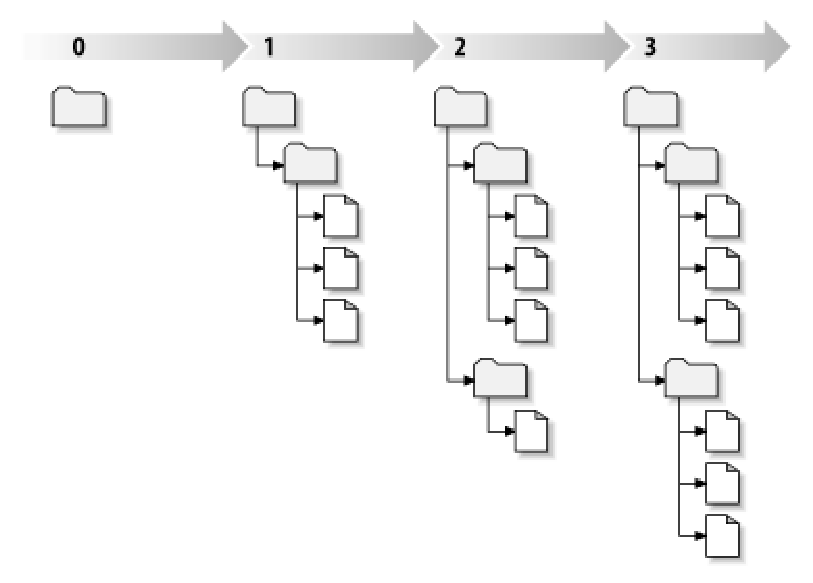
\includegraphics[scale=0.49]{svn_evolution.eps} 
	\end{figure}

	\begin{tabbing}
		---------------------------------------- \= -------------- \= ... \kill
		\> Figura 2.1. Linea de tiempo.
	\end{tabbing}
	}
	\end{frame}
\section{C\'omo se trabaja con SVN?}	
	\begin{frame}{Creando el repositorio}
	\scriptsize
	{	            
	\begin{tabbing}
	Los ejemplos se muestran en un formato CLI (l'{i}nea de comandos) con el cliente \\
	UNIX, pero como se mostrar'a m'as adelante tiene completo soporte de entorno grafico \\
	para MS Windows a trav'es de la aplicaci'on TortoiseSVN.\\ 

	\= -- \= -----\= ---------------------------------------------\=  ... \kill
	\> En la ra'{i}z del servidor de desarrollo se crea la estructura base donde se importaran		\\
	\> los proyectos, esta estructura es virtual y solo contiene la base de datos del repositorio 	\\
	\> y tambi'en los usuarios y permisos con los que opera. \\ \\
	\>\> svnadmin create - -fs-type fsfs /repositorio		 \\	\\
	\>\> ls -l /repositorio/ \\
	\>\> total 8 \\
	\= -- \= ---------------\= ----------------- \= --------\= ... \kill
	\>\> drwxr-xr-x    \> 2 svn svn 128 2009-08-20 11:02 conf \\
	\>\> drwxr-sr-x    \> 6 svn svn 352 2009-08-20 11:02 db \\
	\>\> -r- -r- -r- - \> 1 svn svn \>2 2009-08-20 11:02 format \\
	\>\> drwxr-xr-x    \> 2 svn svn 360 2009-08-20 11:02 hooks \\
	\>\> drwxr-xr-x    \> 2 svn svn 104 2009-08-20 11:02 locks \\
	\>\> -rw-r- -r- -  \> 1 svn svn 229 2009-08-20 11:02 README.txt \\

	\end{tabbing}
	}
	\end{frame}
	
	\begin{frame}{Importar un sistema}
	\scriptsize
	{
	\begin{tabbing}
	Cuando se importa por primera vez un proyecto indicamos el directorio que lo contiene, \\
	donde previamente creamos la estructura con los directorios que requiere el proyecto. \\
	Lo recomendado son los directorios \scriptsize{\color{Blue}src, bin, doc}, etc. \\ \\
	\= -- \= -----\= ---------------------------------------------\=  ... \kill
	\>\> svn import \scriptsize{\color{Blue}directorio\_local} svn://devel.jp.cl/\scriptsize{\color{Blue}nombre\_proyecto}/trunk -m "\scriptsize{\color{Blue}Importaci'on inicial}"	\\ \\
	
	
	\end{tabbing}
	}
	\end{frame}

	\begin{frame}{Exportar un sistema}
	\scriptsize
	{
	\begin{tabbing}
	Hacer un pedido (\scriptsize{\color{Blue}checkout}), consiste en traer la rama de desarrollo en la que se quiere \\
	trabajar solo se ejecuta cuando no existe una copia local del proyecto. \\ \\
	
	Si recurrimos al ejemplo \scriptsize{\color{Blue}palms} para hacer un checkout en el directorio local \scriptsize{\color{Blue}venta\_movil}.  \\ \\
	Seria similar a: \\ \\
	\= -- \= -----\= ---------------------------------------------\=  ... \kill
	\>\> svn checkout svn://devel.jp.cl/palms/trunk \scriptsize{\color{Blue}venta\_movil}	\\ \\
	
	Ahora se tiene la versi'on de desarrollo actual de palms localmente como venta\_movil. \\
	A continuacion veremos como se actualizan los archivos modificados concurrentemente.\\
	\end{tabbing}
	}
	\end{frame}
	
	\begin{frame}{Actualizar un proyecto}

	\scriptsize
	{
	\begin{tabbing}
	Un h'abito fundamental el usar este sistema es la el uso de \scriptsize{\color{Blue}update} esta instrucci'on \\
	suma cualquier cambio enviado al servidor a las modificaciones locales por lo tanto \\
	es de suma importancia ejecutarlo siempre antes de enviar modificaciones al repositorio. \\ \\
	
	\= -- \= -----\= ---------------------------------------------\=  ... \kill
	\>\> svn update \scriptsize{\color{Blue}venta\_movil} 								\\ \\
	
	El ejemplo anterior es la instrucci'on que actualiza una copia del proyecto versionado en \\
	una estaci'on de trabajo.\\
	
	\end{tabbing}
	}
	\end{frame}	
	
	\begin{frame}{Actualizar un proyecto}
	\scriptsize
	{
	\begin{tabbing}
	Para publicar sus cambios para los dem'as, puede utilizar el comando \\
	de Subversion \scriptsize{\color{Blue}commit}. \\ \\
	\= -- \= -----\= ---------------------------------------------\=  ... \kill
	\>\> svn commit \scriptsize{\color{Blue}venta\_movil} 								\\ \\
	
	Ahora que sus cambios a cualquier archivo modificado se han confirmado \\
	en el respositorio, si cualquier otro usuario obtiene una copia de trabajo de\\
	\scriptsize{\color{Blue}venta\_movil}, ver'an sus	cambios en la 'ultima versi'on del archivo.\\
	\end{tabbing}
	}
	\end{frame}	

	\begin{frame}{Ver el log}
	\scriptsize
	{
	\begin{tabbing}
	\= -- \= -----\= ---------------------------------------------\=  ... \kill
	\>\> svn log venta\_movil/							\\
	\>\> - - - - - - - - - - - - - - - - - - - - - - - - - - - - - - - - - - - - - - - - - - - - - - - - - - - -\\
	\>\> r3 | fdiaz | 2008-05-15 23:09:28 -0500 (Thu, 15 May 2008) | 1 line\\ \\
	
	\>\> correcci'on del editar oc\\
	\>\> - - - - - - - - - - - - - - - - - - - - - - - - - - - - - - - - - - - - - - - - - - - - - - - - - - - -\\
	\>\> r2 | fdiaz | 2008-05-14 18:43:15 -0500 (Wed, 14 May 2008) | 3 line\\
	\>\> - - - - - - - - - - - - - - - - - - - - - - - - - - - - - - - - - - - - - - - - - - - - - - - - - - - -\\
	\>\> r3 | cnavarro | 2008-05-15 23:09:28 -0500 (Thu, 15 May 2008) | 1 line\\ \\

	\>\> correcci'on en el metodo guardar cambios\\
	\>\> - - - - - - - - - - - - - - - - - - - - - - - - - - - - - - - - - - - - - - - - - - - - - - - - - - - -\\
	\>\> r2 | cnavarro | 2008-05-14 18:43:15 -0500 (Wed, 14 May 2008) | 6 line\\ \\

	\>\> egregado metodo main() \\
	\>\> - - - - - - - - - - - - - - - - - - - - - - - - - - - - - - - - - - - - - - - - - - - - - - - - - - - -\\
	\>\> r1 | fdiaz | 2008-05-10 19:50:31 -0500 (Sat, 10 May 2008) | 5 line\\ \\

	\>\> Import inicial\\
	\>\> - - - - - - - - - - - - - - - - - - - - - - - - - - - - - - - - - - - - - - - - - - - - - - - - - - - -\\
	\end{tabbing}
	}
	\end{frame}	
	

\section{Muestra del GUI}
	\begin{frame}{Men'us svn en Windows}
	\scriptsize
	{
	\begin{tabbing}
		Graficamente obtendremos todas las opciones CLI.
	\end{tabbing}
	\begin{figure}
	\centering 
		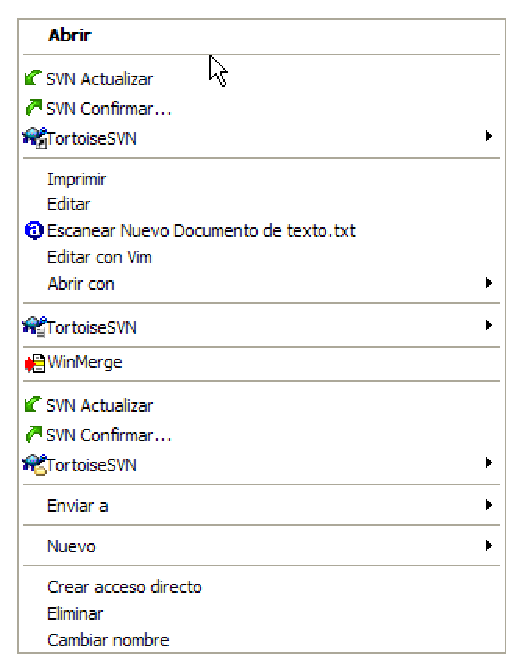
\includegraphics[scale=0.49]{svn_menu.eps} 
	\end{figure}

	\begin{tabbing}
		----------------------- \= -------------- \= ... \kill
		\> Figura 4.1. Men'u integrado a Windows Explorer.
	\end{tabbing}
	}
	\end{frame}
	
	\begin{frame}{Men'u de Opciones}
	\scriptsize
	{
	\begin{tabbing}
		Todas las opciones antes mencionadas estar'an disponibles en los archivos versionados.\\
		Con un simple clic de bot'on derecho en el directorio o archivo.
	\end{tabbing}
	\begin{figure}
	\centering 
		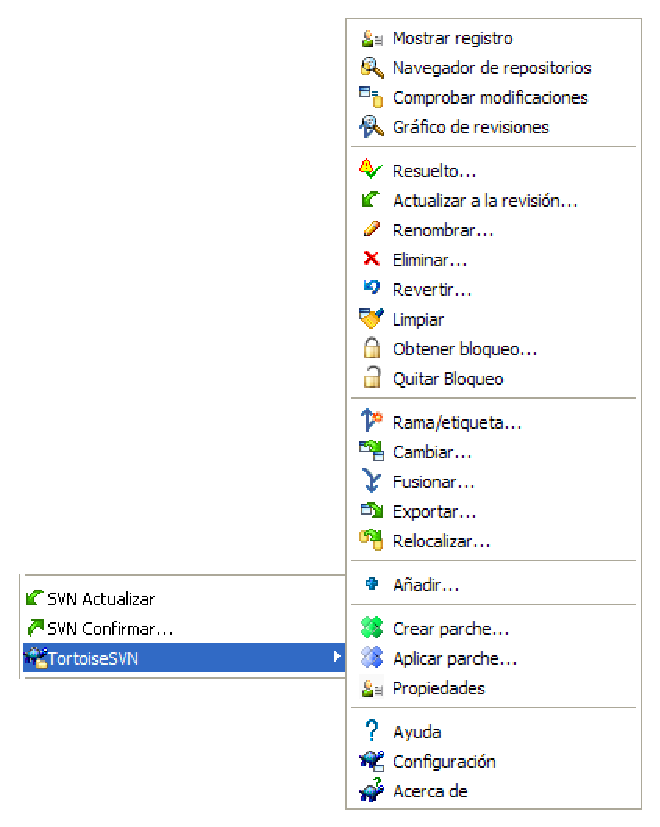
\includegraphics[scale=0.46]{svn_menu_sobre_repo.eps}
	\end{figure}
	\begin{tabbing}
		----------------------- \= -------------- \= ... \kill
		\> Figura 4.2. Men'u contextual para un directorio\\
		\>\> bajo el control de versiones.
	\end{tabbing}
	}
	\end{frame}		
	\begin{frame}{Iconos identificadores para MS Windows}
	\scriptsize
	{
	\begin{figure}
	\centering 
		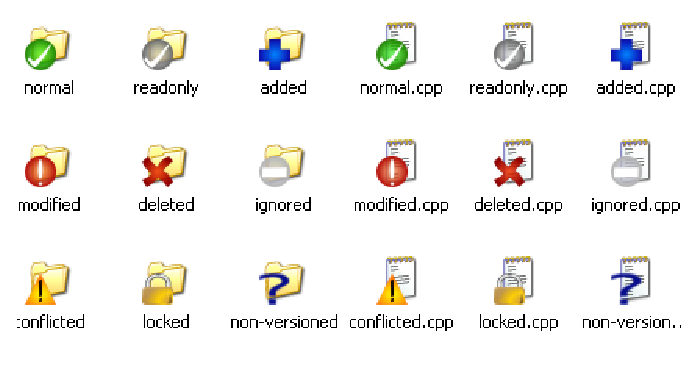
\includegraphics[scale=0.49]{svn_icons.eps}
	\end{figure}
	\begin{tabbing}
		------------ \= --------------- \= ... \kill
		\> Figura 4.3. Conjunto de Iconos que toman los archivos y directorios\\
		\>\>  bajo elsistema de control de versiones.\\
	\end{tabbing}
	}
	\end{frame}	

	\begin{frame}{Estadistica Grafica con TortoiseSVN}
	\scriptsize
	{
	\begin{figure}
	\centering 
		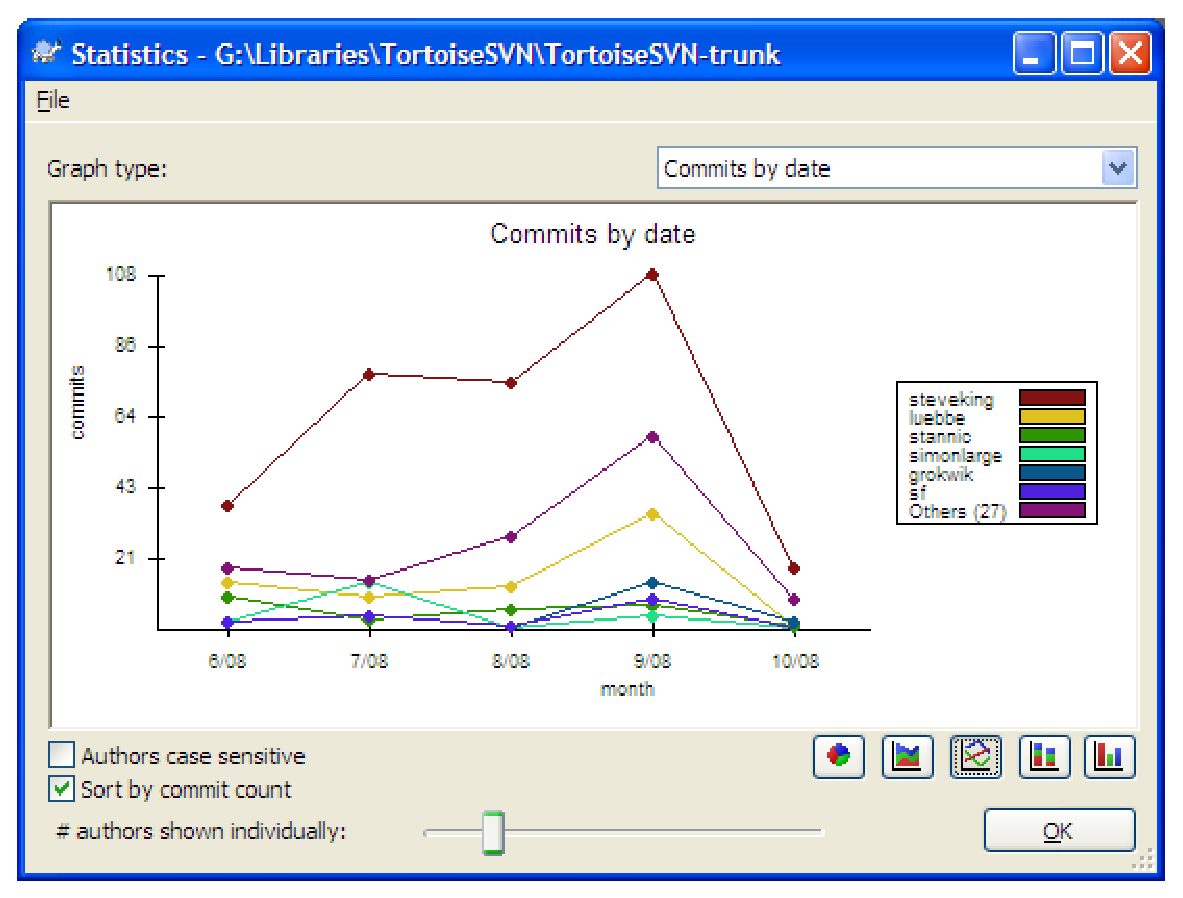
\includegraphics[scale=0.37]{svn_grafico.eps} 
	\end{figure}
	\begin{tabbing}
		----------------------- \= --------------- \= ... \kill
		\>\> Figura 4.4. Graficos por fecha.
	\end{tabbing}
	}
	\end{frame}	
\section{Concluci\'on}	
	\begin{frame}{Concluci'on}
	\scriptsize
	{
	\begin{tabbing}
	En conclusi'on el implantar esta metodolog'{i}a de trabajo, genera fuertes beneficios \\
	en la gesti'on del desarrollo de software, como en las polticas operativas para realizar \\
	el despligu'e de las  aplicaciones. Sumado a lo anterior, obtendremos un fuerte apoyo \\
	estad'{i}stico sobre los proyectos en desarrollo y el trabajo individual de los desarrolladores. \\
	\\
	Por otro lado el proceso de respaldo del c'odigo ser'a mucho m'as optimo. \\
	\\
	El jefe de desarrollo podr'a entregar acceso restringido a los niveles del c'odigo adem'as \\
	de separar el c'odigo y las aplicaciones de los datos que manipulan.\\
	\\
	El desarrollador podr'a gestionar su historial de c'odigo sin afectar la integridad de este \\
	en el tiempo. 

	\end{tabbing}
	}
	\end{frame}
\section{Fin}	
	\begin{frame}{\begin{center} Comentarios \end{center}}

	\end{frame}
	
	\begin{frame}{\begin{center} Gracias \end{center}}

	\end{frame}
\end{document}
